

In this section the detailed schedule is presented as Gantt diagram.\\
It's important to mention that the schedule was made taking into account that the project will be done by professional full-time workers. This said that the documentation part of the project should be done in fewer days than it actually was. However number of hours for each documentation part is the average number of hours our team actually spent.\\
Some diagrams are cut in order to mantain readability.\\
 
	\begin{figure}[h]
		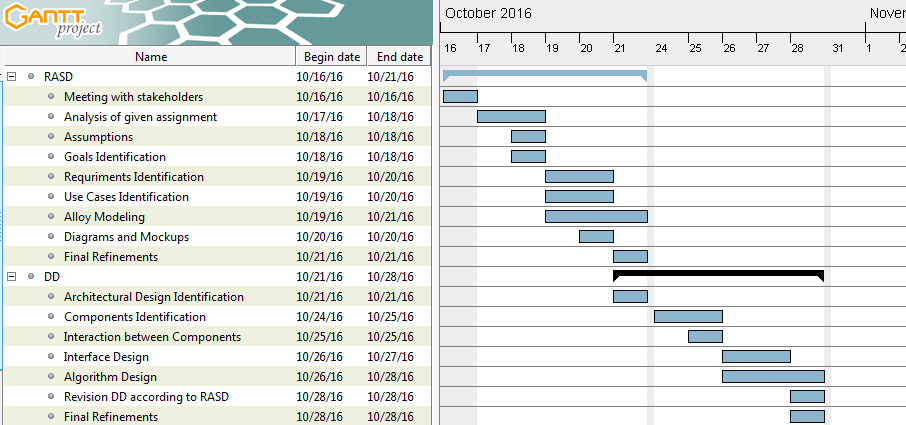
\includegraphics[scale=0.55]{img/Sched1.png}
		\caption{Schedule for RASD and DD parts}
	\end{figure}
\newpage
	\begin{figure}[h]
		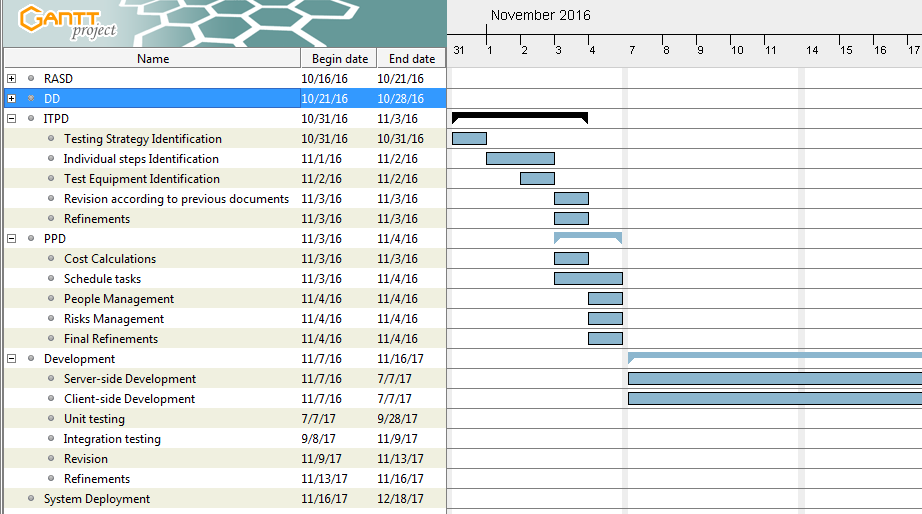
\includegraphics[scale=0.55]{img/Sched2.png}
		\caption{Schedule for ITPD and PP parts}
	\end{figure}
	\begin{figure}[h]
		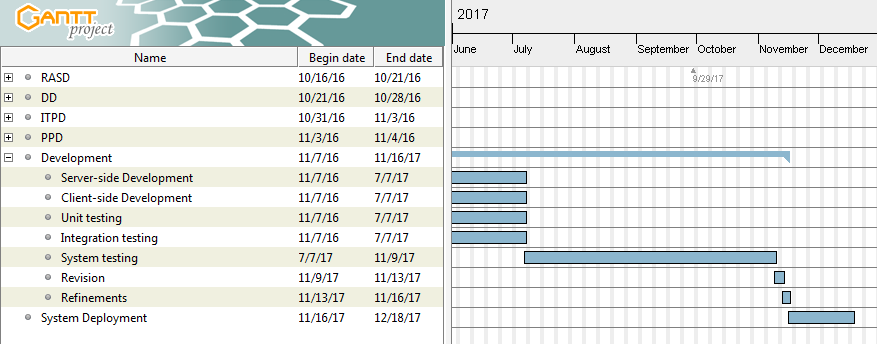
\includegraphics[scale=0.55]{img/Sched3.png}
		\caption{Schedule for Development and System Deployment parts}
	\end{figure}